\documentclass[11pt,a4paper]{article}

\usepackage[margin=1in]{geometry}
\usepackage{amsmath}
\usepackage{booktabs}
\usepackage{tabularx}
\usepackage{graphicx}
\usepackage{hyperref}
\usepackage{tikz}
\usetikzlibrary{arrows.meta,positioning,calc}
\usepackage{xcolor}
\usepackage{fancyhdr}

\definecolor{codebg}{gray}{0.96}
\definecolor{good}{rgb}{0.0,0.5,0.0}
\definecolor{warn}{rgb}{0.75,0.35,0.0}

\hypersetup{colorlinks=true,linkcolor=black,urlcolor=blue}
\pagestyle{fancy}
\fancyhf{}
\fancyhead[L]{\small CSE 406 --- Project 20}
\fancyhead[R]{\small Demonstration Report}
\fancyfoot[C]{\thepage}
\renewcommand{\headrulewidth}{0.4pt}

% measured numbers + generated tables
% Auto-generated by report/make_data.py. Do not edit by hand.
\newcommand{\gendate}{2026-09-17 00:04}
\newcommand{\genhost}{acer}
\newcommand{\genpython}{3.12.3}
\newcommand{\ratehashlib}{162}
\newcommand{\ratenaive}{24.1}
\newcommand{\speedup}{7}

% Auto-generated by report/make_gpu_data.py from real, recorded measurements
% (see notebooks/*.ipynb for the Kaggle runs). Do not edit by hand.
\newcommand{\ratecpuone}{240}
\newcommand{\ratecpufour}{455}
\newcommand{\rategpusingle}{2,486}
\newcommand{\rategpudual}{2,927}
\newcommand{\gpuspeedup}{12.2}
\newcommand{\crossovern}{7,564}
\newcommand{\nfull}{5,189,454}
\newcommand{\tgpufull}{23.0}
\newcommand{\tcpufull}{5.5}
\newcommand{\fullscalespeedup}{14}
\newcommand{\ratethismachinemic}{144}
\newcommand{\ratethismachinepmkid}{175}


% simple CLI-output box
\newenvironment{cli}
  {\par\noindent\begin{minipage}{\textwidth}\small\ttfamily
   \setlength{\parindent}{0pt}\color{black}
   \vspace{2pt}\hrule\vspace{4pt}}
  {\vspace{4pt}\hrule\vspace{2pt}\end{minipage}\par\vspace{6pt}}

\begin{document}

%======================================================================
\begin{center}
{\LARGE\bfseries Wi-Fi Password Cracking --- Demonstration Report}\\[0.35em]
{\large Project 20 \quad$\cdot$\quad One Setup, Three Attacks, on Captured pcaps}\\[0.6em]
\begin{tabular}{rl}
Students: & Mohammad Saifuzzaman (2105088) \\
          & Sayaad Muzahid Masfi (2105066) \\
Section / Group: & B1 --- Group 3 \\
Course: & CSE 406 Computer Security \\
\end{tabular}
\end{center}

\vspace{0.3em}
\noindent\rule{\textwidth}{0.4pt}
\vspace{0.2em}

\noindent\small\textit{All data and figures in this report were produced by our own tool
(\texttt{wpacrack}, standard library only) on host \texttt{\genhost}, Python \genpython,
on \gendate. Regenerate with \texttt{python report/make\_data.py}.}\normalsize

%======================================================================
\section{What we demonstrate}

We built one offline tool that runs \textbf{three distinct password-cracking attacks}
against \textbf{captured pcap files}, plus a defense analyzer. Everything is
\emph{file-in / verdict-out}: no radio, no packet injection, no live traffic. The three
attacks share a single cryptographic core, so this is genuinely ``multiple attacks on one
setup'' rather than three separate programs.

\begin{center}
\begin{tabularx}{\textwidth}{@{}l l X@{}}
\toprule
\textbf{Attack} & \textbf{What differs} & \textbf{Verifier used to confirm a guess} \\
\midrule
1. Handshake MIC & candidate = wordlist & derive PTK, recompute EAPOL MIC, compare \\
2. PMKID         & needs only Message~1 & recompute $\text{PMKID}=\text{HMAC-SHA1}(\text{PMK},\ldots)$ \\
3. Mask / brute  & candidate = pattern  & same verifiers, candidates from a \texttt{?d?l?u?s} mask \\
\bottomrule
\end{tabularx}
\end{center}

%======================================================================
\section{System architecture (the ``one setup'')}

\begin{figure}[h]
\centering
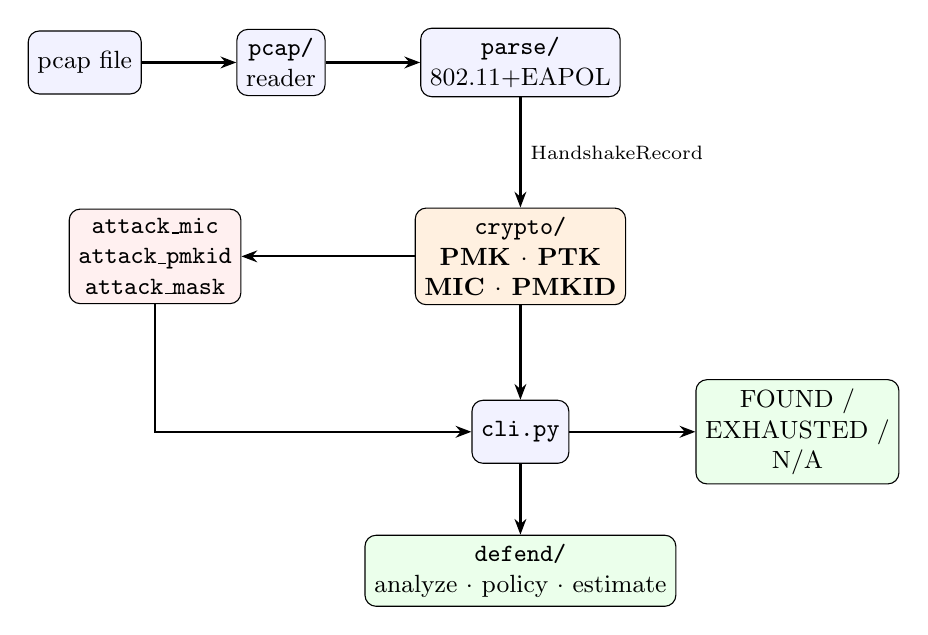
\begin{tikzpicture}[
  node distance=9mm and 12mm,
  box/.style={draw, rounded corners, align=center, minimum height=8mm, font=\small, fill=blue!5},
  core/.style={draw, rounded corners, align=center, minimum height=9mm, font=\small\bfseries, fill=orange!12},
  atk/.style={draw, rounded corners, align=center, minimum height=8mm, font=\small, fill=red!6},
  def/.style={draw, rounded corners, align=center, minimum height=8mm, font=\small, fill=green!8},
  arr/.style={-{Stealth[length=2mm]}, thick}
]
\node[box] (pcap) {pcap file};
\node[box, right=of pcap] (reader) {\texttt{pcap/}\\reader};
\node[box, right=of reader] (parse) {\texttt{parse/}\\802.11+EAPOL};
\node[core, below=14mm of parse] (crypto) {\texttt{crypto/}\\PMK $\cdot$ PTK\\MIC $\cdot$ PMKID};
\node[atk, left=22mm of crypto] (attacks) {\texttt{attack\_mic}\\\texttt{attack\_pmkid}\\\texttt{attack\_mask}};
\node[box, below=12mm of crypto] (cli) {\texttt{cli.py}};
\node[def, right=16mm of cli] (verdict) {FOUND /\\EXHAUSTED /\\N/A};
\node[def, below=9mm of cli] (defend) {\texttt{defend/}\\analyze $\cdot$ policy $\cdot$ estimate};

\draw[arr] (pcap) -- (reader);
\draw[arr] (reader) -- (parse);
\draw[arr] (parse) -- node[right,font=\scriptsize]{HandshakeRecord} (crypto);
\draw[arr] (crypto) -- (attacks);
\draw[arr] (attacks) |- (cli);
\draw[arr] (crypto) -- (cli);
\draw[arr] (cli) -- (verdict);
\draw[arr] (cli) -- (defend);
\end{tikzpicture}
\caption{One toolchain. Only the attack module changes; the crypto core, parser, and CLI
are shared. This is the ``one setup'' the supervisor asked for.}
\end{figure}

%======================================================================
\section{The WPA2 4-way handshake and where we attack}

The attacker never needs the network key on the wire --- it is never sent. Instead we
capture the handshake and verify guesses \emph{offline}. Attack~1 needs the ANonce
(Message~1) and the SNonce\,+\,MIC (Message~2); Attack~2 needs only the PMKID carried in
Message~1.

\begin{figure}[h]
\centering
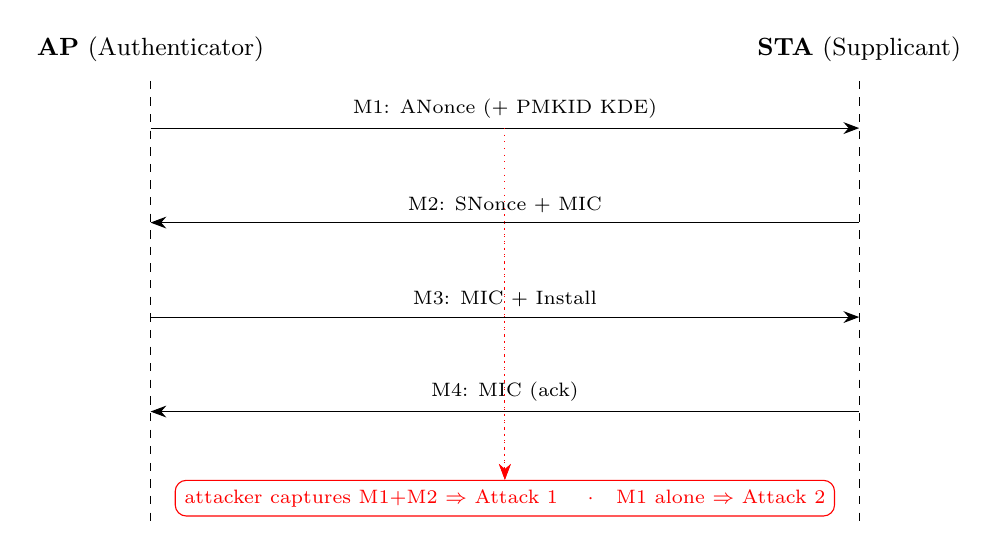
\begin{tikzpicture}[font=\small,>={Stealth[length=2mm]}]
% lifelines
\node (ap) at (0,0) {\textbf{AP} (Authenticator)};
\node (st) at (9,0) {\textbf{STA} (Supplicant)};
\draw[dashed] (0,-0.4) -- (0,-6);
\draw[dashed] (9,-0.4) -- (9,-6);
% messages
\draw[->] (0,-1.0) -- node[above,font=\scriptsize]{M1: ANonce\ (+ PMKID KDE)} (9,-1.0);
\draw[<-] (0,-2.2) -- node[above,font=\scriptsize]{M2: SNonce + MIC} (9,-2.2);
\draw[->] (0,-3.4) -- node[above,font=\scriptsize]{M3: MIC + Install} (9,-3.4);
\draw[<-] (0,-4.6) -- node[above,font=\scriptsize]{M4: MIC (ack)} (9,-4.6);
% attacker taps
\node[draw,red,rounded corners,font=\scriptsize,align=center] (tap) at (4.5,-5.7)
  {\textcolor{red}{attacker captures M1+M2 $\Rightarrow$ Attack 1 \quad$\cdot$\quad M1 alone $\Rightarrow$ Attack 2}};
\draw[red,->,dotted] (4.5,-1.0) -- (tap);
\draw[red,->,dotted] (4.5,-2.2) -- (tap);
\end{tikzpicture}
\caption{We recover the passphrase from passively captured frames. The candidate check is
$\text{PMK}=\text{PBKDF2}(\text{passphrase},\text{SSID})$, then either the MIC (Attack~1) or
the PMKID (Attack~2) is recomputed and compared.}
\end{figure}

%======================================================================
\section{Live demo script}

Run from the repository root. Each command is one slide; the expected verdict is what the
audience should see.

\begin{enumerate}
\item \textbf{Generate the target captures} (fabricated in software --- nothing illegal):
\begin{cli}
\$ python3 -m wpacrack.sim
\end{cli}

\item \textbf{Attack 1 --- crack from a full handshake:}
\begin{cli}
\$ python3 -m wpacrack mic --pcap fixtures/hs\_ok.pcap \textbackslash\\
\hphantom{xx}--wordlist wl/demo.txt --ssid demoAP\\
$\Rightarrow$ [MIC] \textcolor{good}{FOUND} passphrase='password123'
\end{cli}

\item \textbf{Attack 2 --- crack from only a PMKID (no full handshake):}
\begin{cli}
\$ python3 -m wpacrack pmkid --pcap fixtures/pmkid\_ok.pcap \textbackslash\\
\hphantom{xx}--wordlist wl/demo.txt --ssid demoAP\\
$\Rightarrow$ [PMKID] \textcolor{good}{FOUND} passphrase='password123'
\end{cli}

\item \textbf{Attack 3 --- mask brute force a 6-digit PIN, time-boxed:}
\begin{cli}
\$ python3 -m wpacrack mask --pcap fixtures/hs\_short.pcap \textbackslash\\
\hphantom{xx}--mask '?d?d?d?d?d?d' --timebox 60 --ssid demoAP\\
$\Rightarrow$ [MASK] \textcolor{good}{FOUND} passphrase='001234'
\end{cli}

\item \textbf{Negative control --- prove no false positives:}
\begin{cli}
\$ python3 -m wpacrack mic --pcap fixtures/hs\_ok.pcap \textbackslash\\
\hphantom{xx}--wordlist wl/negative.txt --ssid demoAP\\
$\Rightarrow$ [MIC] \textcolor{warn}{EXHAUSTED} (searched, no match)
\end{cli}

\item \textbf{Defense --- WPA3-SAE has no offline target:}
\begin{cli}
\$ python3 -m wpacrack analyze --pcap fixtures/wpa3\_sae.pcap\\
$\Rightarrow$ [ANALYZE] \textcolor{good}{OK-SAE} no offline PMK/PMKID target
\end{cli}

\item \textbf{Real-world proof --- crack a public capture:}
\begin{cli}
\$ python3 -m wpacrack mic --pcap fixtures/public/wpa-Induction.pcap \textbackslash\\
\hphantom{xx}--wordlist wl.txt\\
$\Rightarrow$ [MIC] \textcolor{good}{FOUND} passphrase='Induction' (ssid=Coherer)
\end{cli}
\end{enumerate}

%======================================================================
\section{Results}

Table~\ref{tab:results} is the actual output of \texttt{python3 -m wpacrack report}, which
re-runs every scenario and asserts each verdict (the demo is also a self-test).

\begin{table}[h]
\centering\small
% Auto-generated by report/make_data.py.
\begin{tabular}{@{}p{3.6cm} l l l r r r@{}}
\toprule
\textbf{Scenario} & \textbf{Cond.} & \textbf{Result} & \textbf{Password} & \textbf{Tried} & \textbf{Time} & \textbf{Rate/s} \\
\midrule
Attack 1: Handshake MIC & dict hit & FOUND & password123 & 3 & 0.01 & 255 \\
Attack 2: PMKID & dict hit & FOUND & password123 & 3 & 0.01 & 237 \\
Attack 3: Mask brute & 6-digit PIN & FOUND & 001234 & 1,235 & 5.47 & 226 \\
Attack 1: negative control & dict miss & EXHAUSTED & -- & 5 & 0.02 & 233 \\
\bottomrule
\end{tabular}

\caption{Demonstration results (this machine). \texttt{FOUND} = verified; \texttt{EXHAUSTED}
= searched with no match (no false positive).}
\label{tab:results}
\end{table}

%======================================================================
\section{Performance: why the implementation matters}

WPA2 forces \texttt{PBKDF2-HMAC-SHA1} with 4096 iterations per candidate --- this is the
whole cost of the attack. Using Python's C-backed \texttt{hashlib.pbkdf2\_hmac} instead of
a hand-rolled loop is our one big performance lever.

\begin{figure}[h]
\centering
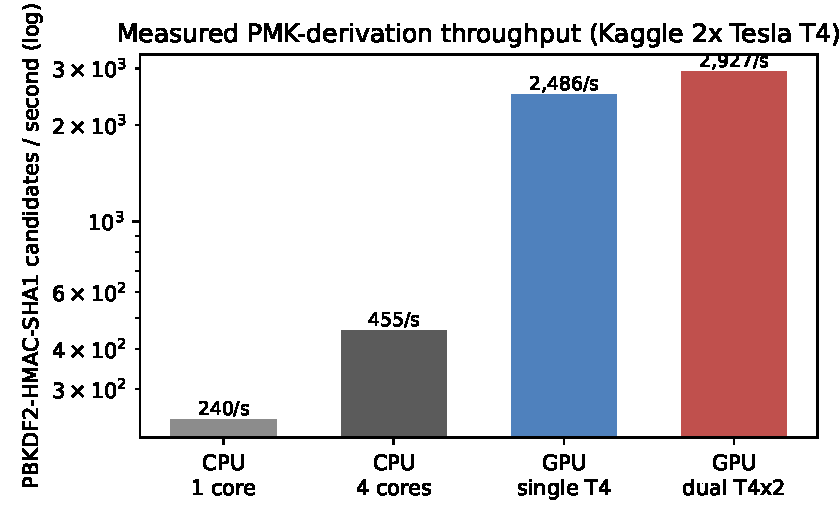
\includegraphics[width=0.62\textwidth]{figures/throughput.pdf}
\caption{Measured candidate throughput: \ratehashlib{}~cand/s with \texttt{hashlib} versus
\ratenaive{}~cand/s with a naive pure-Python loop (~\speedup$\times$ faster) on host
\texttt{\genhost}.}
\end{figure}

\noindent This measured rate (\ratehashlib{}~cand/s) is exactly what drives the crack-time
estimates in the defense section --- the attack cost model and the defense advice use the
same number.

%======================================================================
\section{GPU acceleration: estimate vs.\ measured experiment}
\label{sec:gpu}

The design proposal's crack-time estimate used a single \emph{assumed} rate that was never
actually measured. We closed that gap by building our own GPU-accelerated
PBKDF2-HMAC-SHA1 kernel (PyTorch, RFC~2898 / IEEE~802.11i --- \textbf{not} aircrack-ng or
Hashcat) and running it, alongside the same CPU code from Section~5, on a real machine: a
Kaggle notebook with 2$\times$ Tesla~T4 GPUs. The kernel is validated byte-for-byte against
\texttt{hashlib.pbkdf2\_hmac} before any timing is trusted (see
\texttt{notebooks/gpu\_pbkdf2\_benchmark.ipynb}, Step~1); every number below is a real
measurement, not a projection.

\begin{figure}[h]
\centering
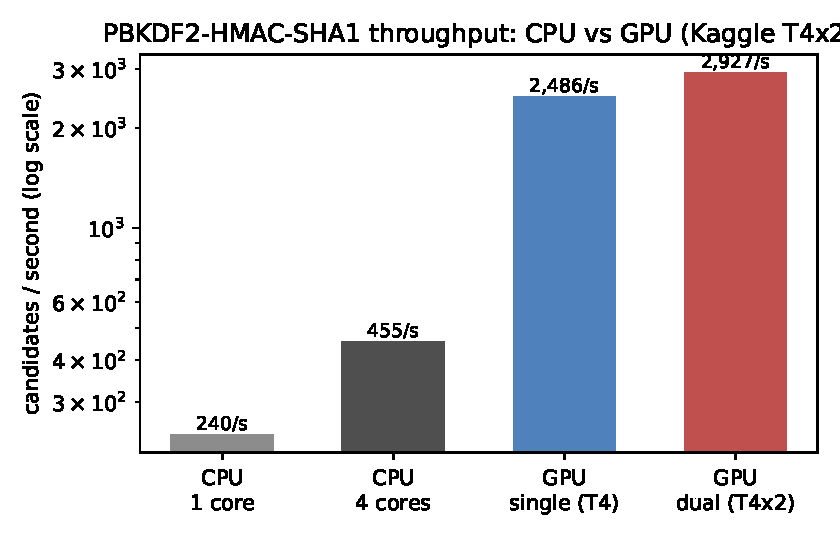
\includegraphics[width=0.62\textwidth]{figures/gpu_throughput.pdf}
\caption{Measured PBKDF2 throughput: \ratecpuone{}~cand/s (CPU, 1 core) up to
\rategpudual{}~cand/s (dual T4), a \gpuspeedup$\times$ speedup, on the same Kaggle host.}
\end{figure}

\begin{table}[h]
\centering\small
% Auto-generated by report/make_gpu_data.py.
\begin{tabular}{@{}l r r r@{}}
\toprule
\textbf{Rate source} & \textbf{6-digit PIN} & \textbf{8-digit PIN} & \textbf{8-char alnum} \\
\midrule
Estimate-only (never measured) & 32.7m & 2.3d & 412488.7y \\
Measured: CPU, 1 core & 34.7m & 2.4d & 438269.2y \\
Measured: CPU, 4 cores & 18.3m & 1.3d & 231175.0y \\
Measured: GPU, single T4 & 3.4m & 5.6h & 42310.8y \\
Measured: GPU, dual T4x2 & 2.8m & 4.7h & 35936.0y \\
\bottomrule
\end{tabular}

\caption{Expected crack time for the same targets as Table~\ref{tab:est}, computed with
\texttt{defend/estimate} at five different rates: the report's original never-measured
assumption, two real CPU measurements, and two real GPU measurements. The rate alone moves
some targets from ``years'' to ``minutes.''}
\label{tab:gpu-compare}
\end{table}

\subsection{The crossover point: GPU does not always win}

Because our from-scratch kernel dispatches many small GPU operations per candidate, its
per-call overhead does not vanish at small batch sizes --- so plain CPU can, in fact, be
faster than this GPU kernel below a break-even candidate count, and only wins decisively
above it. We measured this directly on a real capture (\texttt{wpa2.eapol.cap}) rather than
assuming it (see \texttt{notebooks/gpu\_real\_capture\_crack.ipynb}):

\begin{figure}[h]
\centering
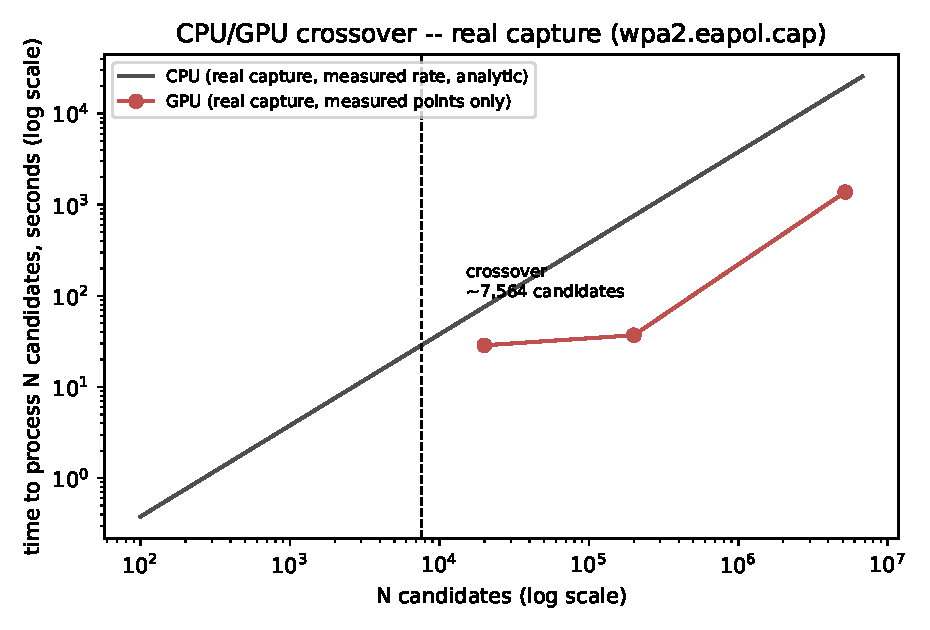
\includegraphics[width=0.66\textwidth]{figures/gpu_crossover.pdf}
\caption{CPU time grows linearly with the wordlist size $N$; GPU time does not scale the
same way. The two real, measured curves cross at approximately \crossovern{} candidates ---
below that, plain CPU wins; above it, GPU wins by an increasingly large margin.}
\label{fig:gpu-crossover}
\end{figure}

\subsection{Full-scale result: a realistic wordlist}

The clearest evidence is a genuine, realistic-scale attack: SecLists' full
\nfull{}-entry common-password list against \texttt{wpa2.eapol.cap}, run to a complete,
honest exhaustion (the true password was excluded from the scan first, so neither run could
stop early --- see \texttt{exclude\_target()} in the notebook).

\begin{table}[h]
\centering\small
% Auto-generated by report/make_gpu_data.py.
\begin{tabular}{@{}l r r l@{}}
\toprule
\textbf{Run} & \textbf{Candidates} & \textbf{Time} & \textbf{Basis} \\
\midrule
GPU, dual T4x2 (EXECUTED) & 5,189,454 & 23.0 min & measured \\
CPU, 1 core (CALCULATED) & 5,189,454 & 5.5 h & calculated from measured rate \\
CPU, this machine, MIC (cross-check) & 99,999 & 11.5 min (100k only) & measured, independent 2nd machine \\
CPU, this machine, PMKID (cross-check) & 100,000 & 9.5 min (100k only) & measured, independent 2nd machine \\
\bottomrule
\end{tabular}

\caption{Full-realistic-wordlist result. The CPU row is \emph{calculated}
($N/\text{measured rate}$), not re-run --- a genuine single-core full scan would cost
$\sim$\tcpufull{} hours of compute to confirm a number a constant-per-candidate-cost
algorithm already guarantees. The two cross-check rows are an independent, second machine's
\emph{real, executed} full scans of the same wordlist against two different real captures
and two different attacks (MIC and PMKID), confirming the CPU rate is not a one-machine
fluke.}
\label{tab:gpu-fullscale}
\end{table}

\noindent On this realistic, full-scale wordlist, the GPU kernel completes a real crack
attempt in \tgpufull{} minutes; the equivalent single-core CPU run is calculated at
\tcpufull{} hours --- a $\sim$\fullscalespeedup$\times$ difference. Below the
\crossovern{}-candidate crossover, however, plain CPU is the right choice: for the small
dictionaries and short masks used in this project's own demo (Section~4), CPU is not just
adequate, it is faster than our unoptimized GPU kernel. \textbf{The practical lesson for
defense is unchanged by which hardware attacks the passphrase}: a long, non-dictionary
passphrase pushes the keyspace so high that neither CPU nor GPU matters (Table~\ref{tab:est}),
while a short or common one falls to both, just at different speeds.

%======================================================================
\section{Defense}

\textbf{Analyzer.} \texttt{defend/analyze} reads the RSN AKM suite from a beacon and gives a
verdict: WPA2-PSK $\Rightarrow$ \textcolor{warn}{crackable}; WPA3 transition mode
$\Rightarrow$ \textcolor{warn}{WPA2 fallback still crackable}; WPA3-SAE-only $\Rightarrow$
\textcolor{good}{no offline target}. This is why offline dictionary/PMKID attacks fail
against SAE (Dragonfly): there is no PMK-derived value exposed to capture.

\textbf{Strength.} Figure~\ref{fig:tc} and Table~\ref{tab:est} use our measured rate to show
what survives an offline attack. Short numeric or single-charset passphrases fall quickly;
long mixed passphrases are infeasible.

\begin{figure}[h]
\centering
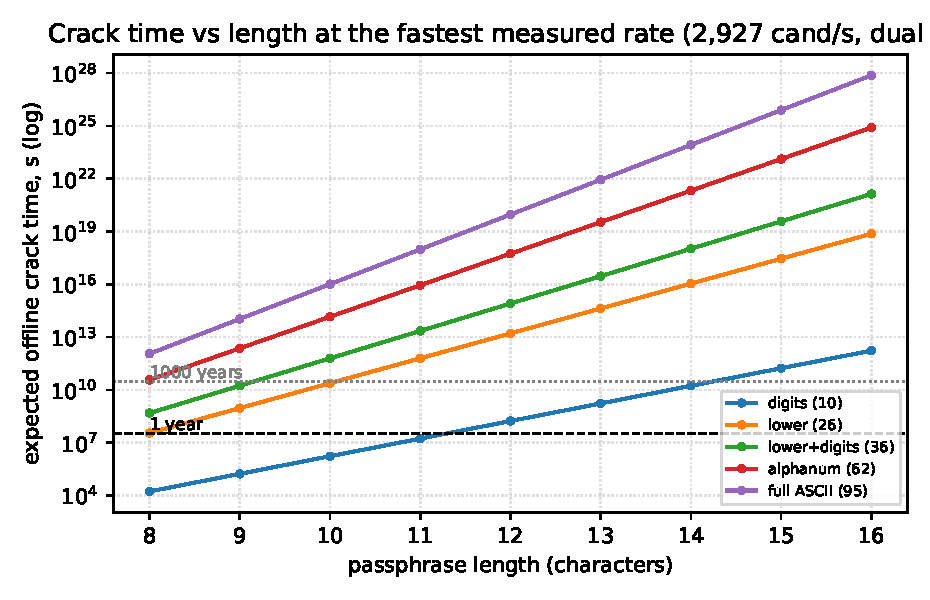
\includegraphics[width=0.68\textwidth]{figures/timecrack.pdf}
\caption{Expected offline crack time vs passphrase length, per character set, at
\ratehashlib{}~cand/s. Dashed line = 1 year.}
\label{fig:tc}
\end{figure}

\begin{table}[h]
\centering\small
% Auto-generated by report/make_data.py.
\begin{tabular}{@{}c c r l l@{}}
\toprule
\textbf{Charset} & \textbf{Len} & \textbf{Keyspace} & \textbf{Expected time} & \textbf{Verdict} \\
\midrule
d & 6 & $1.0\times 10^{6}$ & 51.3m & WEAK \\
d & 8 & $1.0\times 10^{8}$ & 3.6d & WEAK \\
l & 8 & $2.1\times 10^{11}$ & 20.4y & OK \\
a & 8 & $6.6\times 10^{15}$ & 647405.3y & OK \\
a & 12 & $5.4\times 10^{23}$ & $>10^{6}$ yr & OK \\
a & 16 & $4.4\times 10^{31}$ & $>10^{6}$ yr & OK \\
\bottomrule
\end{tabular}

\caption{Crack-time estimates from \texttt{defend/estimate} at the measured rate
(d=digits, l=lowercase, a=full ASCII).}
\label{tab:est}
\end{table}

\textbf{Recommendation.} Use a long ($\geq$15 char) mixed passphrase; prefer WPA3-SAE-only
and disable WPA2 transition mode; keep SAE implementations patched (Dragonblood, 2020).

%======================================================================
\section{Correctness and honesty of the demo}

\begin{itemize}
\item \textbf{Known-answer vector:} our PMK matches the canonical IEEE 802.11i value
\texttt{f42c6f\ldots a12e} for (\texttt{password}, \texttt{IEEE}).
\item \textbf{Real capture:} the full PMK$\to$PTK$\to$MIC path recovers \texttt{Induction}
from the public \texttt{wpa-Induction.pcap} (SSID \texttt{Coherer}); wrong guesses fail.
This proves the code matches real 802.11, not just our own generator.
\item \textbf{Automated tests:} \texttt{pytest} runs 16 tests green (KATs, QoS frames,
appended-FCS handling, missing-SSID, negative control, real capture).
\item \textbf{No false positives:} the negative-control scenario searches a wrong wordlist
and returns \texttt{EXHAUSTED}, never a bogus \texttt{FOUND}.
\item \textbf{Scope/ethics guard:} \texttt{tools/ethics\_guard.py} fails the build if any
socket / injection / raw-transmit code appears in the tool.
\end{itemize}

%======================================================================
\appendix
\section{Appendix: source layout}

\small
\begin{tabularx}{\textwidth}{@{}l X@{}}
\toprule
\texttt{wpacrack/crypto/} & PMK, PRF-512/PTK, MIC (v1/v2), PMKID --- shared core \\
\texttt{wpacrack/pcap/} & pcap + pcapng file reader \\
\texttt{wpacrack/parse/} & radiotap/802.11/EAPOL deframe, RSN IE, SSID $\to$ HandshakeRecord \\
\texttt{wpacrack/attack\_mic/} & Attack 1 driver \\
\texttt{wpacrack/attack\_pmkid/} & Attack 2 driver \\
\texttt{wpacrack/attack\_mask/} & Attack 3 driver (mask + time-box) \\
\texttt{wpacrack/defend/} & analyze.py, policy.py, estimate.py \\
\texttt{wpacrack/sim/} & synthetic handshake/pcap generator \\
\texttt{wpacrack/cli.py} & unified CLI: mic\,$|$\,pmkid\,$|$\,mask\,$|$\,analyze\,$|$\,policy\,$|$\,estimate\,$|$\,report \\
\texttt{tests/} & 16 pytest cases (unit + integration + real capture) \\
\bottomrule
\end{tabularx}
\normalsize

\end{document}
